\documentclass[pdftex,11pt,a4paper]{article}
\usepackage{blindtext}
\usepackage{graphicx}
\usepackage{subfiles}
\usepackage{amsmath}
\usepackage{amsthm}
\usepackage{tikz}
\usepackage{wrapfig}
\usepackage{lscape}
\usepackage{rotating}
\usepackage{epstopdf}
\usepackage{subcaption}
\usepackage[font=small,labelfont=bf]{caption}
\usepackage{hyperref}
\usepackage{color}
\usepackage{algorithm}% http://ctan.org/pkg/algorithms
\usepackage{algpseudocode}% http://ctan.org/pkg/algorithmicx
\hypersetup{
    colorlinks=true,
    linkcolor=blue,
    citecolor=blue
}
\usetikzlibrary{shapes.geometric, arrows}
\theoremstyle{definition}
\newtheorem{definition}{Definition}[section]
\newtheorem{theorem}{Theorem}[section]
\newtheorem{lemma}[theorem]{Lemma}
\theoremstyle{remark}
\newtheorem*{remark}{Remark}
\usepackage{amssymb}
\usepackage{amsfonts}
\usepackage{mathtools}
\usepackage{geometry}
 \geometry{
 a4paper,
 total={210mm,297mm},
 left=30mm,
 right=30mm,
 top=30mm,
 bottom=35mm,
 }
\newcommand{\defeq}{\vcentcolon=}
\newcommand{\eqdef}{=\vcentcolon}
\newcommand*{\V}[1]{\mathbf{#1}}%
\newcommand{\norm}[1]{\left\lVert#1\right\rVert}
\newcommand{\justif}[2]{&{#1}&\text{#2}}
\newcommand{\qedwhite}{\hfill \ensuremath{\Box}}
\newcommand\given[1][]{\:#1\vert\:}
\newcommand{\me}{\mathrm{e}}
\DeclarePairedDelimiterX{\infdivx}[2]{(}{)}{%
  #1\;\delimsize\|\;#2%
}
\DeclarePairedDelimiter\abs{\lvert}{\rvert}%
\newcommand{\Conv}{\mathop{\scalebox{1.5}{\raisebox{-0.2ex}{$\ast$}}}}%
\newcommand{\infdiv}{\infdivx}
\renewcommand{\qed}{\hfill\blacksquare}
\hyphenation{op-tical net-works semi-conduc-tor tech-no-lo-gy}


\begin{document}
\title{A length-invariant method to build relational structures from birdsong}
\author{Bernardo P\'erez Orozco\\University of Oxford\\\texttt{ber@robots.ox.ac.uk} \and Davide Zilli \\University of Oxford\\\texttt{dzilli@robots.ox.ac.uk} \and Katherine J. Willis \\ University of Oxford \\ \texttt{kathy.willis@zoo.ox.ac.uk} \and Stephen J. Roberts\\University of Oxford\\\texttt{sjrob@robots.ox.ac.uk}}

\maketitle


\begin{abstract}
In this work, we propose a length-invariant method to build hierarchical relational structures from time series. We propose summarising a set of time series as a set of Variational Hidden Markov Models, which appropriately learn information from the symbols and temporal structure contained in the dataset. Then, we define a similarity metric based on the log-likelihood of observing specific sequences in a given model. Afterwards, the output distance matrix is used in Agglomerative Hierarchical Clustering so as to generate the relational structure. To demonstrate the use of our method, we set out an experiment to build a \textit{phylo-acoustic tree} of bird species, i.e. a structure displaying the acoustic relations across bird species in a hierarchical fashion. Finally, we evaluate our experiment by showing that the generated trees do exhibit a clear community structure by comparing them with null hypothesis trees.
\end{abstract}


\section{Introduction}
\label{section_introduction}
The explosion of data in recent years has allowed scientists to gain insight in a diversity of domains. Furthermore, the widespread use of computational methods has in turn provided means of rapidly extracting conclusions from data. In this work, we tackle the problem of building hierarchical structures from time series. Importantly, characterising time series introduces the problem of dealing with sequences of different length, which in itself is also a problem of information redundancy, i.e. longer sequences may contain repeated patterns that do not translate into information gain.
\par In this work, we propose a length-invariant method to produce such relational structures: we first train a Variational Hidden Markov Model (HMM) over a feature time series and then compare them using a novel similarity metric based on sequence generation likelihood. This enables us to use Agglomerative Hierarchical Clustering to build a relational structure. In particular, our experimental setting consists in building a \textit{phylo-acoustic tree} of bird species, i.e. a hierarchical structure that summarises acoustic relations across a wide range of bird species.
\par Phylo-acoustic structures may have little in common with their genetic counterparts, which do not account for exogenous phenomena. Even though birdsong is learnt by repetition, forced migration may push flocks to learn songs that do not necessarily come from their parents \cite{Berwick2013}. Birdsong is also hierarchical and regular \cite{Snowdon2013}, i.e. it is composed of motifs of patterns as can be seen in Figure \ref{fig_birdsong_structure}, and hence the amount of information in individual songs is dominated by the number of different patterns that appear, and not by their number of occurrences. 

\begin{figure}[t]
\centering
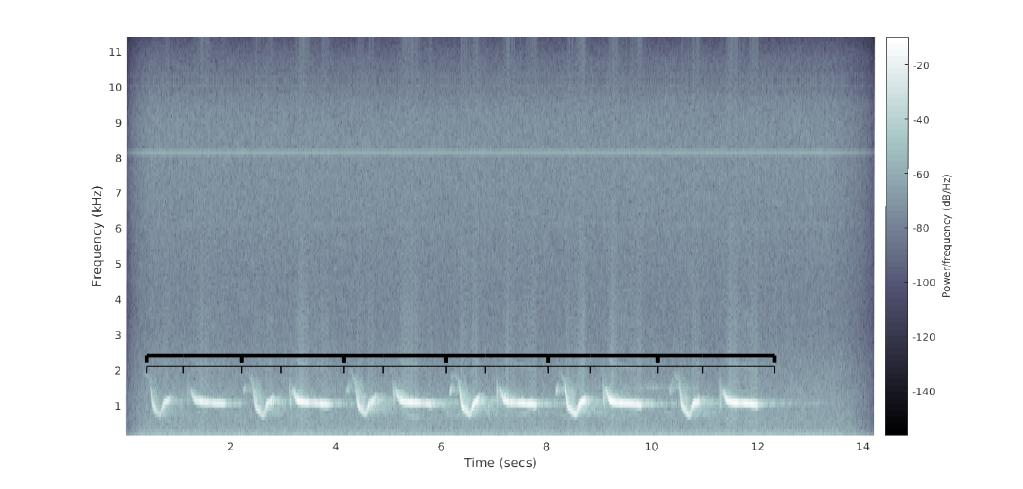
\includegraphics[width=\textwidth]{images/birdsong_structure.jpg}
\caption{Spectrogram of a birdsong recording of the species \emph{Periparus ater}. Note the regular structure of birdsong: syllables (thick boxes) are composed of motifs (thin boxes).}
\label{fig_birdsong_structure}
\end{figure}

\par The rest of this article is organised as follows: first, in Section \ref{section_review} we provide a literature review on building relational structures from time series; then in Section \ref{section_model}, we introduce the mathematical framework used to build such structures; in Section \ref{section_results}, we present our experiments and results; and in Section \ref{section_conclusion} we present our conclusions and future work.

\section{Literature review}
\label{section_review}
The main challenge is to define a similarity metric for HMMs that allows for an even comparison between trajectories. As a result the method will have been endowed with length-invariance, which can be seen as characterising the source of the time series.
\par Some methods used in the literature to handle comparisons between vectors of different length include Dynamic Time Warping (DTW) \cite{Jancovic2013,Muda2010} and zero-padding (i.e. ignoring the longer portion in the long recording, thus heavily affecting similarity for recordings with radically different durations); we are concerned with characterising the source of the time series, so neither DTW nor zero-padding address this issue directly. Moreover, these methods do not allow for a fair comparison between signals that have the same motif instantiated a different number of times. This raises the need to train models that correctly learn not only the symbols, but also the temporal dynamics of the signal. One such model is the HMM.
\par However, the literature on HMM similarity is not broad. The authors in \cite{Lyngs1999} define a similarity metric in terms of the co-emission probability (i.e. the probability of generating the same sequence of observations independently); \cite{Bahlmann2001} uses the Bayes Probability of Error instead, which can be understood as the area of overlap of two densities $p_1, p_2$ with priors $\pi_1, \pi_2$ under the restriction $\pi_1+\pi_2 = 1$; finally, a third distance measure is proposed in \cite{Juang1985} for discrete HMMs, and consists in computing the norm between their emission models, which are empirical probability density functions (pdfs). Nevertheless, these methods all focus on a subset of the parameters of the HMM (namely, the emission model's parameters), and therefore leave out the information given by the temporal dynamics of the signal.
\par More recent approaches attempt to define the metric in terms of the sequence-generation likelihood obtained during the decoding phase of the HMM, which incorporates both the information contained in each observed symbol, and the temporal structure of the sequence of observations. For example, \cite{Bicego,Smyth} define the distance between two HMMs $\lambda_p, \lambda_q$ as a linear function of the log-likelihood of observing a particular sequence $\V{x}$ (associated to the first model) using the second one $\lambda_q$.
\par However, this last approach still relies completely on a single, absolute contribution made by one HMM when decoding a sequence. Instead, in \cite{Porikli2004} the authors propose to make a distance metric that combines not only the training sequences $\V{x}_p, \V{x}_q$ used to train the models $\lambda_p, \lambda_q$, but also the performance of the models on each other's training sequence, i.e. the contributions given by the log-likelihoods $\text{LL}(\V{x}_p \given \lambda_q), \text{LL}(\V{x}_q \given \lambda_p)$. Nevertheless, their approach does not account for the numerical dominance that any of these factors could exhibit in practice.
\par One last approach in the literature is to build the relational structure without explicitly computing a distance matrix. For example, the work in \cite{Coviello2014} develops a novel algorithm called ``Variational Hierarchical Expectation-Maximisation" that computes cluster centres on the run. Nevertheless, we are interested in developing a modular method in such a way that its different components can be reused, e.g. by directly defining a distance metric (as opposed to developing a specialised algorithm), we will be able to use a wider range of clustering and visualisation methods.  
\par Therefore, in our work we will aim at defining an HMM distance metric that addresses the shortcomings described above. In particular, we will address the need for defining a metric that comprises information from both the transition and emission models while also considering the performance of the HMMs in sequences other than its own training sequence.


%Birdsong analysis has long been of interest in the research community because it encapsulates behavioural information that can be extracted by means of tools with a formal mathematical background. For example, birdsong analysis has been used extensively to perform bird species classification \cite{Chou2009,Wielgat2012,McIlraith1995,Lee2013,Franzen2003,Silla2013}, which consists in fitting a model that is able to tell what species unseen birdsong excerpts belong to.
%\par More generally, problems such as bird species classification and birdsong syllable segmentation have also motivated the search for optimal feature representations of birdsong. Crucially, much research has pointed out the similarities between human speech and birdsong \cite{Snowdon2013,McIlraith1995}, which has enabled scientists to use methods from the speech recognition domain to analyse birdsong.
%\par Some of the techniques frequently used in the literature to extract features from birdsong are: Mel-Frequency Cepstral Coefficients \cite{Silla2013,Wielgat2012,Stowell2014,Lopes2011}, raw Mel spectra \cite{Stowell2014} and wavelets \cite{Chou2009}. Other techniques used in the domain of Automated Speech Recognition include formant trajectory extraction \cite{Prica2010,Welling1998}.
%\par One key remark is that these techniques are not length-invariant: they all produce feature representations that vary in length proportionally to the length of the original signal. This is a scalability issue that must be addressed in order to allow for faithful comparison across bird species. In particular, we seek to characterise bird species and not just birdsong recordings. This implies that recordings of radically different lengths should still be considered similar if they were both produced by the same species. This motivates the search for length-invariant comparison methods.

%\par The state of the art suggests that there exists little work on environment quantification by means of birdsong statistical analysis. In \cite{Collins2009}, the authors have used ANOVA to analyse the relation between birdsong, migration strategy and divergent sexual selection. In addition, \cite{BolhuisJohanJ.andEveraertMartin2015} suggests a testable scenario for song evolution by describing acoustic and syntactic differences in bird behavioural traits, such as female responses to song complexity, effects of cross-fostering and identification of regional variations in birdsong.
%\par Finally, to the authors' best knowledge, there is no work on building hierarchical similarity structures by means of birdsong analysis. Therefore, these results can be used to improve existing applications of birdsong analysis, e.g. one such tree can be used as prior knowledge to build an \emph{in situ} bird species classifier.

 

\section{Model architecture}
\label{section_model}
In this section, we describe a procedure to build hierarchical relational structures given a dataset $\mathcal{D}$ with time series produced by different sources from a set $X$. We are interested in finding a relation $R$ over pairs of elements in $X$, along with a scalar $d_{i, j} \in \mathbb{R}$ called the \emph{similarity} between species $s_i, s_j \in S$, i.e. $R \subseteq S \times S \times \mathbb{R}$. This relation can then be expressed as a symmetric matrix $A = (d_{i,j})$ and be used as input to build a hierarchical structure by means of Agglomerative Hierarchical Clustering (AHC). 
\par We aim to characterise each source $s_i$ in a length-invariant fashion, and we do so by training a Variational Hidden Markov Model over its corresponding time series $\V{f} \in \mathcal{D}$. These HMMs are then compared via a similarity metric and the resulting distance matrix is used as input for AHC to produce the final structure. In this section, we will introduce formant trajectory extraction, which results from an application of the Linear Predictive Coding framework. This will be relevant in our experimental setting. We will also introduce the Variational Bayes HMM framework, and a novel metric to measure their similarity.

\subsection{Feature extraction}
Many techniques exist in the literature to extract features from acoustic signals, most of which have been motivated by research in the field of human speech recognition. These include Mel-frequency Cepstral Coefficients \cite{Jurafsky2009, Chou2008a, Stowell2014, Gutierrez-Osuna2009}, which have also been used in combination with spherical K-means \cite{Stowell2014}, the MUSIC algorithm \cite{Evans, Kootsookos1999} and wavelets \cite{Gamulkiewicz2003, Chou2009}.
\par In this work, we are interested in extracting sequences of features that are compact and that have a solid mathematical framework based on how birdsong is produced. Crucially, the features we extract should also shed light on the source that generates the original data (which in this case are the bird species themselves). This is a key aspect that methods such as MFCCs do not possess, since they are based on sound perception, as opposed to sound production.
\par Formant trajectory extraction is a technique based on the source-filter model of speech production \cite{Snell1993}, which models the vocal tract of the source in a compact manner, and hence yields a formal mathematical underpinning to model birdsong production.
\par Consider a short excerpt (20-40ms) of birdsong $\V{s}$. Now, assume that this short segment of birdsong recording $\V{s}$ can be approximated by a $p$-th order autoregressive model $\hat{\V{s}}$ with $\hat{s}_n = \sum_{i=1}^pa_is_{n-i}$. This prediction has an error $\V{e}$ given by:
\begin{align*}
e_n = s_n - \hat{s}_n = s_n - \sum_{i=1}^pa_is_{n-i}
\end{align*}
The error $\V{e}$ can also be seen as the output of a Linear Time-invariant (LTI) system whose filter subtracts the best approximation $\hat{\V{s}}$ from $\V{s}$ \cite{Bello}, and its system function can be found by taking the z-transform of the equation above: 
\begin{align*}
\mathcal{Z}\{\V{e}\} &= \mathcal{Z}\{\V{s} - \hat{\V{s}}\}\\
E(z) &= S(z) - S(z)\sum_{i=1}^pa_iz^{-i}\\
 &= S(z)A(z)
\end{align*}
\par where $A(z) = 1 - \sum_{i=1}^pa_iz^{-i}$ is the system function. Now, consider the inverse LTI system with input $\V{e}$, output $\V{s}$ and system function $H(z)$. Then, $H(z)A(z) = 1$ and hence:
\begin{align*}
H(z) = \frac{1}{1-\sum_{i=1}^pa_iz^{-i}}
\end{align*}
where the $(a_i)_{i=1}^p$ are the coefficients of the p-th order autoregressive model associated to the birdsong approximation $\hat{\V{s}}$. Crucially, remark that this LTI system is fully characterised by the coefficients $a_i$. 
\par We now define the formant frequencies of the excerpt $\V{s}$ as the poles of the system function $H(z)$; intuitively, these can be thought of as the resonances of the vocal tract \cite{Prica2010} when generating birdsong. Now, given a pair of complex roots $re^{\pm\theta i}$, the formant frequency in Hertz associated to it is given by:
\begin{align*}
F = \frac{f_s}{2\pi}\theta
\end{align*}
where $f_s$ is the sampling frequency of the signal. Furthermore, its 3 dB bandwidth in Hertz is:
\begin{align*}
B = -\frac{f_s}{2\pi}\log{r}
\end{align*}
\par Formants can also be interpreted intuitively as the peaks of the spectral envelope of the signal \cite{Darch}. Smaller bandwidths hint at clearer, more characteristic formants. By framing the original birdsong recording into small excerpts and repeating the procedure above, we obtain a trajectory of formants extracted uniformly over small intervals of time. Figure \ref{fig_specformants} shows the trajectory of the first non-zero formant for a birdsong recording.

\begin{figure}[t]
\centering
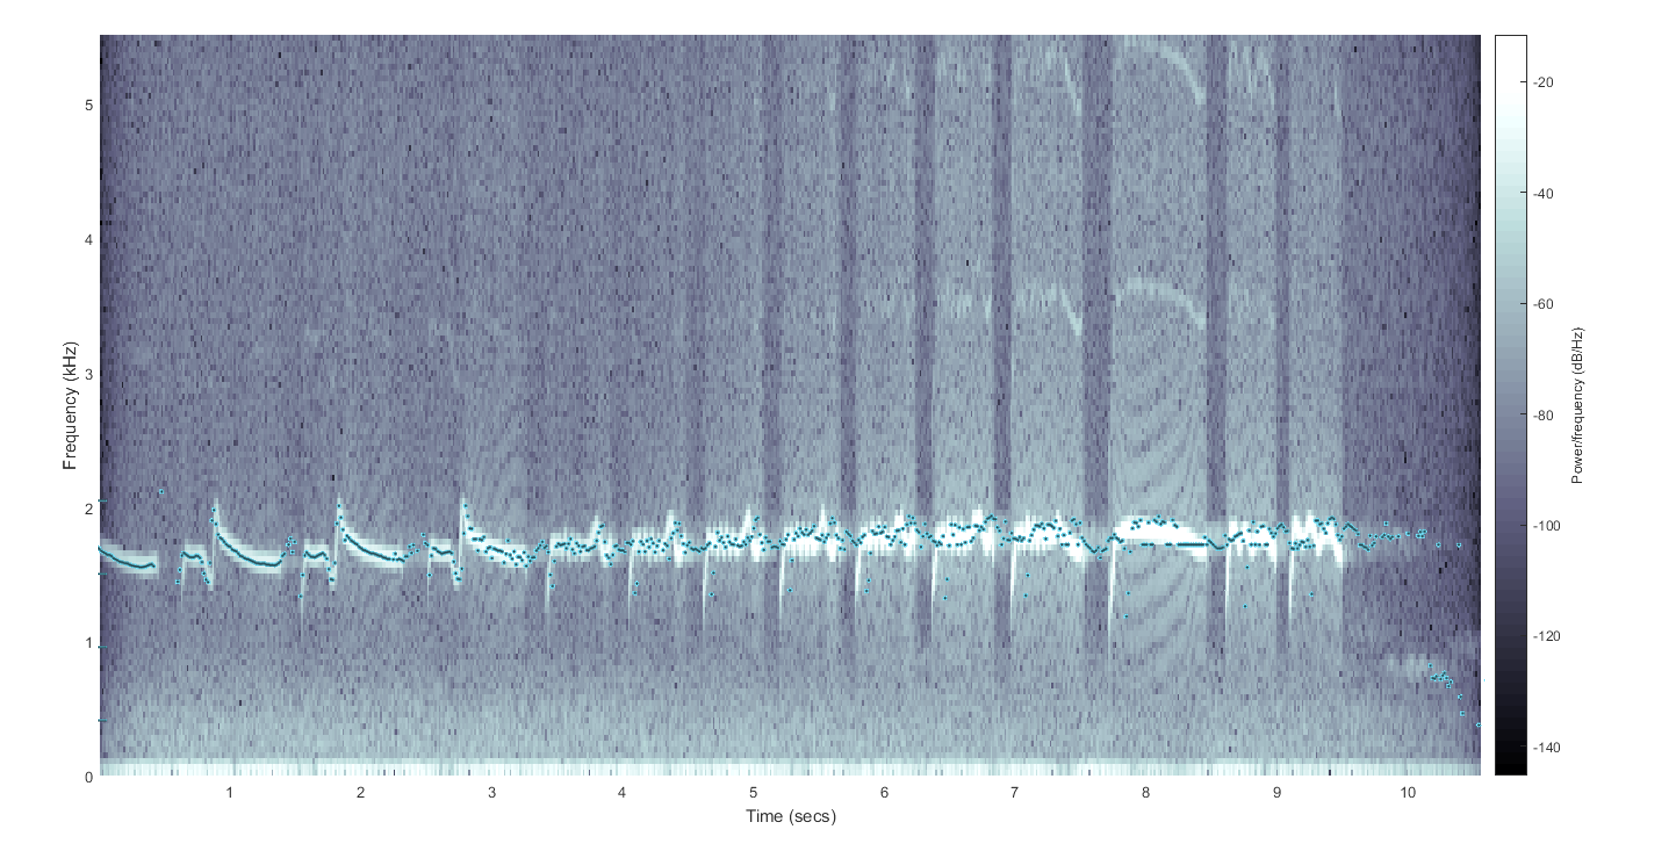
\includegraphics[width=\textwidth]{images/formants}
\caption{Depiction of the first non-zero formant trajectories (blue) on top of a birdsong recording spectrogram of the species \emph{Periparus ater}. Remark how the trajectory corresponds to the white bands (sections with a larger amount of energy) of the spectrogram.}
\label{fig_specformants}
\end{figure}

\subsection{Variational Bayes Hidden Markov Models} \label{sub_hmms}
Once each time series has been transformed into a feature representation, we can train models that characterise each of their sources. Recall that this step endows our approach with the length-invariance property, which is crucial in order to capture similarities across different sources. We now present the Variational Bayes Hidden Markov Models (VB-HMM), which are the key component in this architecture.

%\subsubsection{Kernel Density Estimation}
%\label{sub_kde}
%\par Kernel Density Estimation (KDE) approximates the probability density function of a set of points as a linear combination of basis functions (non-negative kernels). We place an instance of this basis function around each point in the set, add them up and normalise. For the univariate case, the pdf $p_K(x)$ obtained from KDE using kernel $K$ over a set of points $X$ is given by:
%\begin{align*}
%p_K(x) = \frac{1}{Nh}\sum_{i=1}^NK\left(\left|\frac{x - x_i}{h}\right|\right)
%\end{align*}
%where $h$ is called the bandwidth. Crucially, using a smooth kernel provides a smooth pdf as a result, where the degree of smoothness is controlled by the parameter $h$, and its value will make the resulting probability function be oversmoothed, undersmoothed or optimally smoothed.
%\par One of the most common smooth kernels in the literature is the univariate Gaussian kernel \cite{hastie2008}, given by:
%\begin{align*}
%K_G\left(\frac{x}{h}\right) = \frac{1}{\sqrt{2\pi}}\exp{\left(-\frac{x^2}{2h^2}\right)}
%\end{align*}
%whose optimal bandwidth in the least-squares error sense is given by $h = \hat{\sigma}n^{-1/5}$, where $\hat{\sigma}$ is the standard deviation of the sample $X$.
%\par Note that, despite its simplicity, KDE is a poorly scalable strategy: on one hand, the bandwidth $h$ becomes harder to choose as the dimensionality of data increases \cite{Hansen2009}; additionally, the space required to store the output pdf increases exponentially with each added dimension.

%\subsubsection{Gaussian Mixture Models}
%\label{subsection_gmm}
%The scalability challenge imposed by KDE motivates the look for a more compact representation of data. Note that formant trajectories for different birdsong syllables from the same species have been shown to exist in different frequency ranges. This suggests the existence of subpopulations in our data $\mathcal{X}$. In this case, we can use a smaller number of basis functions. This can be achieved by means of a Gaussian Mixture Model (GMM), which is a convex combination of Gaussians (called \emph{mixtures}). In other words, the pdf fitted to the data takes the form:
%\begin{equation} \label{eq:mixmod}
%p(\V{x} \given \theta ) = \sum_{i=1}^K\pi_i \mathcal{N}(\V{\mu}_i, \Sigma_i) 
%\end{equation}
%with $\sum_i=1^K\pi_i, 0 \leq \pi_i\leq 1$. Nevertheless, even if GMMs are more scalable than KDE, neither method allows for the existence of time ordering of data. That is, both models treat the formant trajectories as sets, rather than sequential structures. This motivates the need for an even more abstract structure that takes into consideration the sequential structure of formant trajectories.

We propose summarising the time series of extracted features as Variational Hidden Markov Models. On one hand, this approach is more powerful than fitting plain probability distributions, since HMMs are not only endowed with an emission model $\phi$ which serves to the same purpose, but they are also capable of capturing time-ordering via a Markov Chain transition model $B$. By describing the values $x_t$ and then describing their temporal dynamics, we can fully describe a sequence $\V{x}$. In addition, a Variational HMM also allows for a natural shrinking of the number of states, which results in a more accurate selection of this configuration parameter. A full treatment of Variational HMMs can be found in \cite{Rezek2005}.
\par In this scenario, we aim to infer the probability that the model generated the time series $\V{x}$ and that the underlying Markov Process generated the sequence of states $\V{s}$. This is given by the joint probability distribution $p(\V{x}, \V{s})$:
\begin{equation}\label{eq:hmm}
p(\V{x}, \V{s}) = p(\V{s})p(\V{x} \given \V{s}) = p(s_1)\prod_{t=1}^{T-1}p(s_{t+1}\given s_t)\prod_{t=1}^Tp(\V{x}_t \given s_t)
\end{equation} 
\par Formant trajectories can be described by an HMM with a continuous observation model, such as a Gaussian Mixture Model (GMM), which is given by a convex combination of Gaussians:
\begin{equation} \label{eq:mixmod}
p(\V{x} \given \theta ) = \sum_{i=1}^K\pi_i \mathcal{N}(\V{\mu}_i, \Sigma_i) 
\end{equation}
\par An HMM is fully characterised by the three parameters $\theta = (\phi, B, \pi)$, where $\pi$ is called the initial state distribution. However, note that for every HMM with $K$ states, there exist $K!$ equivalent HMMs that can be generated by permuting the identities of the HMM's states. This is called the \emph{identifiability} problem \cite{Bishop2006}.
\par We now address HMM training. We aim to make inferences about the parameters $\theta$ given data $\mathcal{X}$. A \emph{frequentist} approach to this is Maximum Likelihood Estimation (MLE). However, MLE has several disadvantages \cite{Murphy2012}. Firstly, there is no measure of uncertainty regarding the point estimate $\hat{\theta}$, and thus we are not able to know how trustworthy the estimate is. Secondly, the mode of a distribution is often untypical \cite{Murphy2012} because it does not take into account the volume distribution of the probability density function. Finally, MLE estimates are prone to overfitting data. 
\par These disadvantages can be treated by performing Bayesian learning. In the Bayesian approach, we measure uncertainty by letting the parameters $\theta$ be probability distributions about which we have beliefs. These are represented by prior distributions. A full treatment of how this framework can be used specifically for continuous HMM training is given in \cite{Rezek2005}, where the posterior distributions for the transition and initial state models are approximated as Dirichlet distributions. The authors also give an account of the emission models for different kinds of observations. In particular, for Gaussian models, they approximate the mean as a Normal Distribution and the precision matrices as Wishart densities. 
\par There is still one more issue to address: model selection, i.e. determining how many states an HMM should have. Although techniques such as cross-validation have been extensively investigated \cite{Siddiqi2007,Rezek2005}, Variational Bayes approaches have been shown to have a natural shrinkage of the number of states, i.e. the state space dimension $K$ need not be estimated by iterative training and testing of models. Instead, the system finds an optimal number of states during training: states not visited by the model collapse and only those that correspond to the true number of clusters are used \cite{Rezek2005}. 

\subsection{Similarity metrics}
We now consider distance metrics between probability distributions and between HMMs, and aim to give some examples of metrics in order to build relational structures.
\par The Symmetric Kullback-Leibler (KL) divergence is a similarity metric for continuous probability densities, which can be approximated for discrete probability distributions $P, Q$ as follows:
\begin{align*}
d_{\text{SKLD}}(P, Q) &= \frac{1}{2}\sum_iP_i\log{\frac{P_i}{Q_i}} + Q_i\log{\frac{Q_i}{P_i}}\\
\end{align*}
\par Closed forms for the KL divergence of some parametric distributions do exist, accounting for a more efficient computation ($\mathcal{O}(1)$) of the metric above. 
\par In this work, we also propose a metric to compare HMMs based on the log-likelihood of observing training sequences. In particular, consider two HMMs $\lambda_p, \lambda_q$ trained on two independent sequences $\V{x}_p, \V{x}_q$, then their relative cross likelihood is given by:
\begin{equation}
d_{\text{RCL}}(\lambda_p, \lambda_q) = \left\lvert\frac{\text{LL}(\V{x}_p \given \lambda_p) - \text{LL}(\V{x}_q \given \lambda_p)}{\text{LL}(\V{x}_p \given \lambda_p)}\right\rvert + \left\lvert\frac{\text{LL}(\V{x}_q \given \lambda_q) - \text{LL}(\V{x}_p \given \lambda_q)}{\text{LL}(\V{x}_q \given \lambda_q)}\right\rvert
\end{equation}
\par This metric addresses the following aspects from the literature: on the one hand, it considers the contributions of both, the emission and transition models by simulating the behaviour of the whole HMM; additionally, it allows for a two-way comparison by pondering how both HMMs fare relative to each other's, in addition to their own, training sequence; finally, by using relative likelihoods (as opposed to plain likelihoods), we also guarantee that both terms are making an equal contribution to the final outcome.


\subsection{Agglomerative Hierarchical clustering}
AHC consists in initialising $N$ singleton clusters from the dataset $\mathcal{X} = \{x_1, x_2, ..., x_N\}$ and progressively merging them until only a single cluster containing all of $\mathcal{X}$ remains. Each level of the hierarchy is a subset of the dataset $\mathcal{X}$, and the number of subsets never increases over time.
\par The AHC algorithm is displayed in algorithm \ref{alg_ahc}. It comprises only two stages: a merging phase, in which the two closest clusters are merged, and a recalculation stage, in which the similarity between the newly created cluster and the rest is recalculated. How the new similarities are computed depends on the linkage method. The three most widely known linkage methods \cite{hastie2008} are described below:
\par Single linkage consists of letting the two clusters $G, H$ be as close as they can be by choosing the distance of their closest elements. In other words:
\begin{align*}
d_{SL} = \min_{i \in G, i' \in H} d_{i, i'}
\end{align*}
Similarly, the complete linkage method chooses the two elements that are the furthest apart:
\begin{align*}
d_{CL} = \max_{i \in G, i' \in H} d_{i, i'}
\end{align*}
Finally, group average clustering instead takes the average distance between each pair:
\begin{align*}
d_{GA} = \frac{1}{\abs{G}\abs{H}}\sum_{i\in G}\sum_{i'\in H}d_{i, i'}
\end{align*}
\begin{algorithm}
\begin{algorithmic}[1]
\Function{AHC}{$X, M$}
\Repeat
\State Merge the two closest clusters
\State Recalculate similarity between the new cluster and the rest
\Until{only a single cluster remains}
\EndFunction
\caption{The Agglomerative Hierarchical Clustering algorithm.}\label{alg_ahc}
\end{algorithmic}
\end{algorithm}
\par Note that all three methods tend to show the same results for data that exhibits clustering tendencies \cite{hastie2008}, i.e. data with well-defined, tight clusters that are themselves located well apart from each other. The result of the AHC algorithm can be visualised in a dendrogram, which is the representation of the resulting arborescent structure. Note that AHC algorithms have a monotonicity property that always guarantees the existence of a dendrogram representation \cite{hastie2008}.

\subsection{Dendrogram divergence}
\label{subsub_divergence}
Finally, we are also concerned by computing the similarity between the structure of two trees $T_i, T_j$. This will enable us to show that our resulting trees do have real structure because they are fundamentally different from trees generated from random data, as will be seen in Subsection \ref{sub_results}.
\par Consider a tree $T$, and let $c(x)$ be the function that gives the number of clusters remaining by stopping Agglomerative Hierarchical Clustering at lifetime $x$, and let $c'(x)$ be its derivative. We now define the divergence between trees $T_i, T_j$ as:
\begin{align*}
d(T_i, T_j) = \norm{c'_i(x) - c'_j(x)}
\end{align*}
Using the derivative enables us to measure how fast clusters form as their lifetime increases; in particular, if both trees $T_i, T_j$ have a similar structure, then the rate of change of cluster formation will be similar in both cases too.

\section{Experiments and results}
\label{section_results}
\subsection{Implementation}
We implemented a system capable of building phylo-acoustic trees automatically. The implementation runs in MATLAB 2016a and all the experiments were executed on an Intel(R) Core(TM) i7-4790 CPU @ 3.60GHz processos, 16 GB RAM,  on Ubuntu 14.04. We used the Animal Sound Archive (ASA) bird vocalisation dataset, which contains 3686 birdsong recordings of more than 100 different bird species from all over Europe \cite{AnimalSoundArchive2015}. We used the data for 82 bird species that had at least 15 seconds of birdsong recording each. All the recordings are in WAV format (i.e. uncompressed) and sampled at 22,500 Hz.
\par We used the following pre-processing before extracting formant trajectories: a pre-emphasis filtering with $\alpha = 0.95$; segmentation into frames of 40 ms with an overlap of 50\% \cite{Stowell2014}; finally, each frame is convolved with a Hamming window to avoid sharp edges. 
\par The number of formants we estimate per window corresponds to the rule of thumb $N_f = f_s / 2000$, where $f_s$ is the sampling frequency of the recording \cite{markel1976}. Since birdsong goes to frequencies as high as 10,000 Hz \cite{Marler2004}, and that we want to have 1 formant per thousand Hz, all the birdsong files must be sampled at least at 20,000 Hz, we chose a conventional 22,500 Hz sampling frequency. Furthermore, the order of the LPC model corresponds to $p = 2N_f + 2$ to account for complex conjugate roots \cite{Benesty}. 
\par Once the formants for a given window have been calculated, all values $f_{i, j} < 500$ Hz are filtered as noise \cite{Stowell2014}, and only the formants with a bandwidth narrower than 500 Hz are kept. 
\begin{figure}[t]
\centering
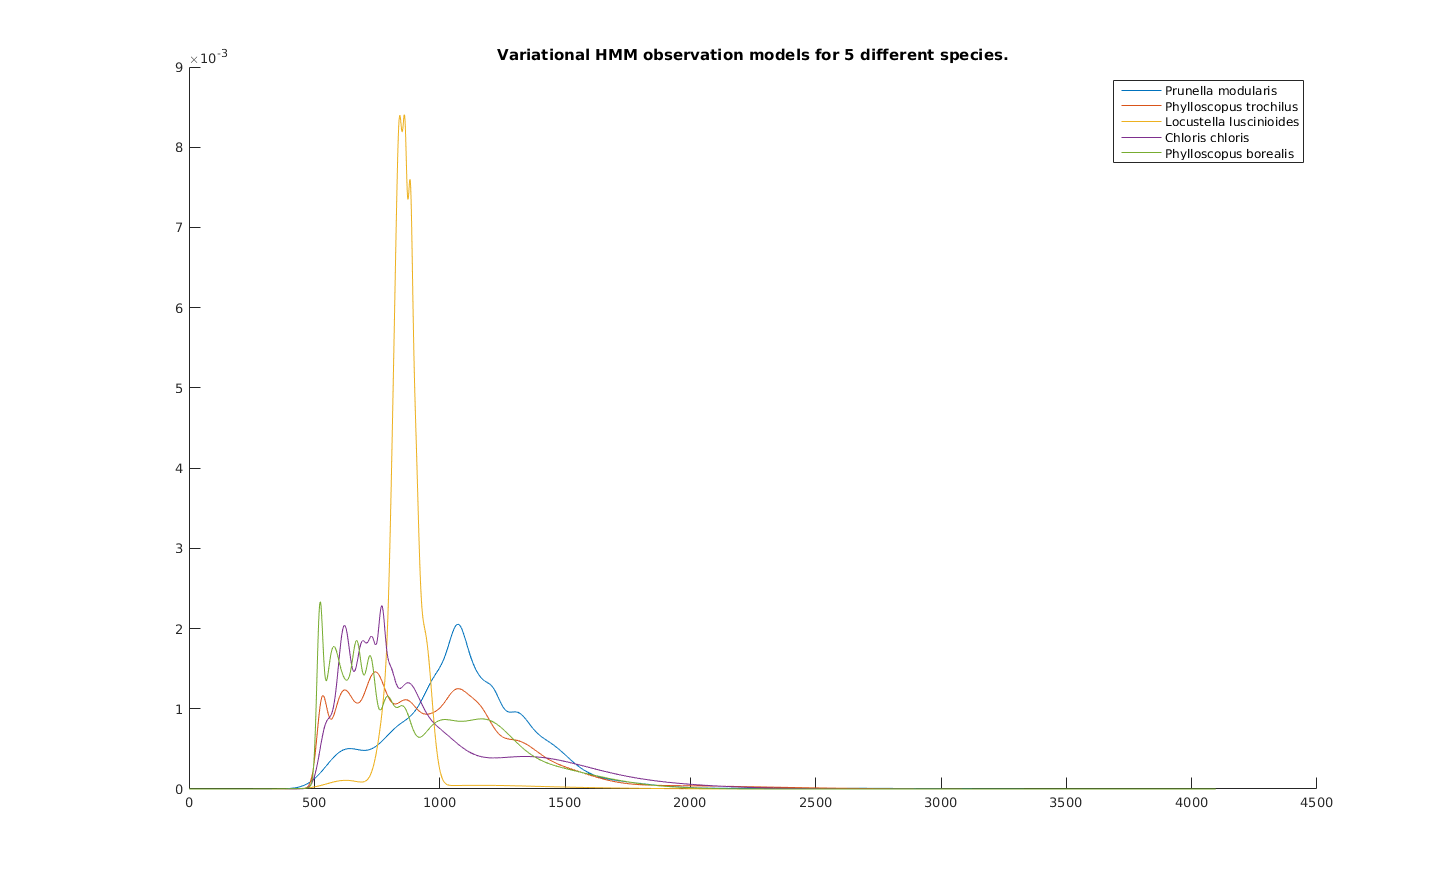
\includegraphics[width=\textwidth]{images/gmm_plots}
\caption{Comparison of HMM observation models for 5 different species. Despite having high probability in similar ranges of frequencies, their shapes are still distinguishable. }
\label{fig_kdespecies}
\end{figure}
\par Concerning VB-HMMs, we used the implementation of the Oxford Machine Learning Research Group, HMMBOX 4.1, which requires the NETLAB package. The former contains implementations of the tools required for a Bayesian treatment of HMMs, in particular: implementation of closed forms for the KL-divergence of the Normal, Dirichlet and Wishart distributions, variational inference training and sequence decoding. Figure \ref{fig_kdespecies} shows the resulting observation models of this procedure for 5 different bird species in the ASA dataset. %Furthermore, a routine that computes the occupancy of an HMM $\Omega_\lambda$ with respect to a sequence $\V{x}$ was also implemented. After computing the formant trajectories for each recording, the ones corresponding to a single species were concatenated and used as the training sequence for each HMM, i.e. we trained one HMM per species, and then computed their occupancy with respect to their respective training sequences. We used a Gaussian observation model for every HMM.
\par All the similarity metrics described in Section \ref{section_model} were implemented as MATLAB scripts as well. Finally, the MATLAB Statistics and Machine Learning Toolbox contains functions to perform agglomerative hierarchical clustering.

\subsection{Results}
\label{sub_results}
We now present phylo-acoustic trees obtained from using the techniques described in Section \ref{section_model}. We used two different approaches to build phylo-acoustic trees:
\begin{itemize}
\item Symmetric KL Divergence over Gaussian Mixture Models trained as emission models of an HMM.
\item Relative Cross Likelihood over Hidden Markov Models.
\end{itemize}
\par We first show that all these trees have true structure by disproving the null hypothesis:
\begin{align*}
H_0 = \text{there is no relationship between the species in a phylo-acoustic tree.}
\end{align*}
\par If this hypothesis is true, then randomly generated data has the same structure as any of these trees. To generate such random data, we sample formant trajectories from the uniform distribution $\mathcal{U}(f_{min}, f_{max})$, where the boundaries of the distribution correspond to the minimum and maximum formant seen in any species in the dataset. After generating as many formant trajectories as bird species, we build new phylo-acoustic trees for each of them.
\par We can now decide which tree exhibits the most structure by computing the divergence (see Subsection \ref{subsub_divergence}) between the trees $T_i, T_{i'}$, which have been generated by using method $i$ from the list above on real data and random data, respectively. The divergence gives a measure on how similar the rates of change between both trees are, hence a tree with a higher divergence from its random counterpart exhibits a clearer structure. The divergences for all six pairs of phylo-acoustic trees are shown in Table \ref{tab1}. Full-size figures of the two phylo-acoustic tree are offered below. 

\begin{table}[t]
\begin{tabular}{r|r|r}
     \textbf{method} &\textbf{divergence}\\
     \hline
     \textbf{Relative cross likelihood over VB-HMM} & 23,896\\
     SKLD over GMMs from VB-HMM & 18,894
\end{tabular} 
\caption{Divergence (as defined in Subsection \ref{subsub_divergence}) between pairs of trees obtained from real data and random data, respectively. The greater the value of the divergence is, the clearer the structure the real data tree has.} \label{tab1}
\end{table}

\begin{sidewaysfigure}[!Ht]
\noindent\makebox[\textwidth]{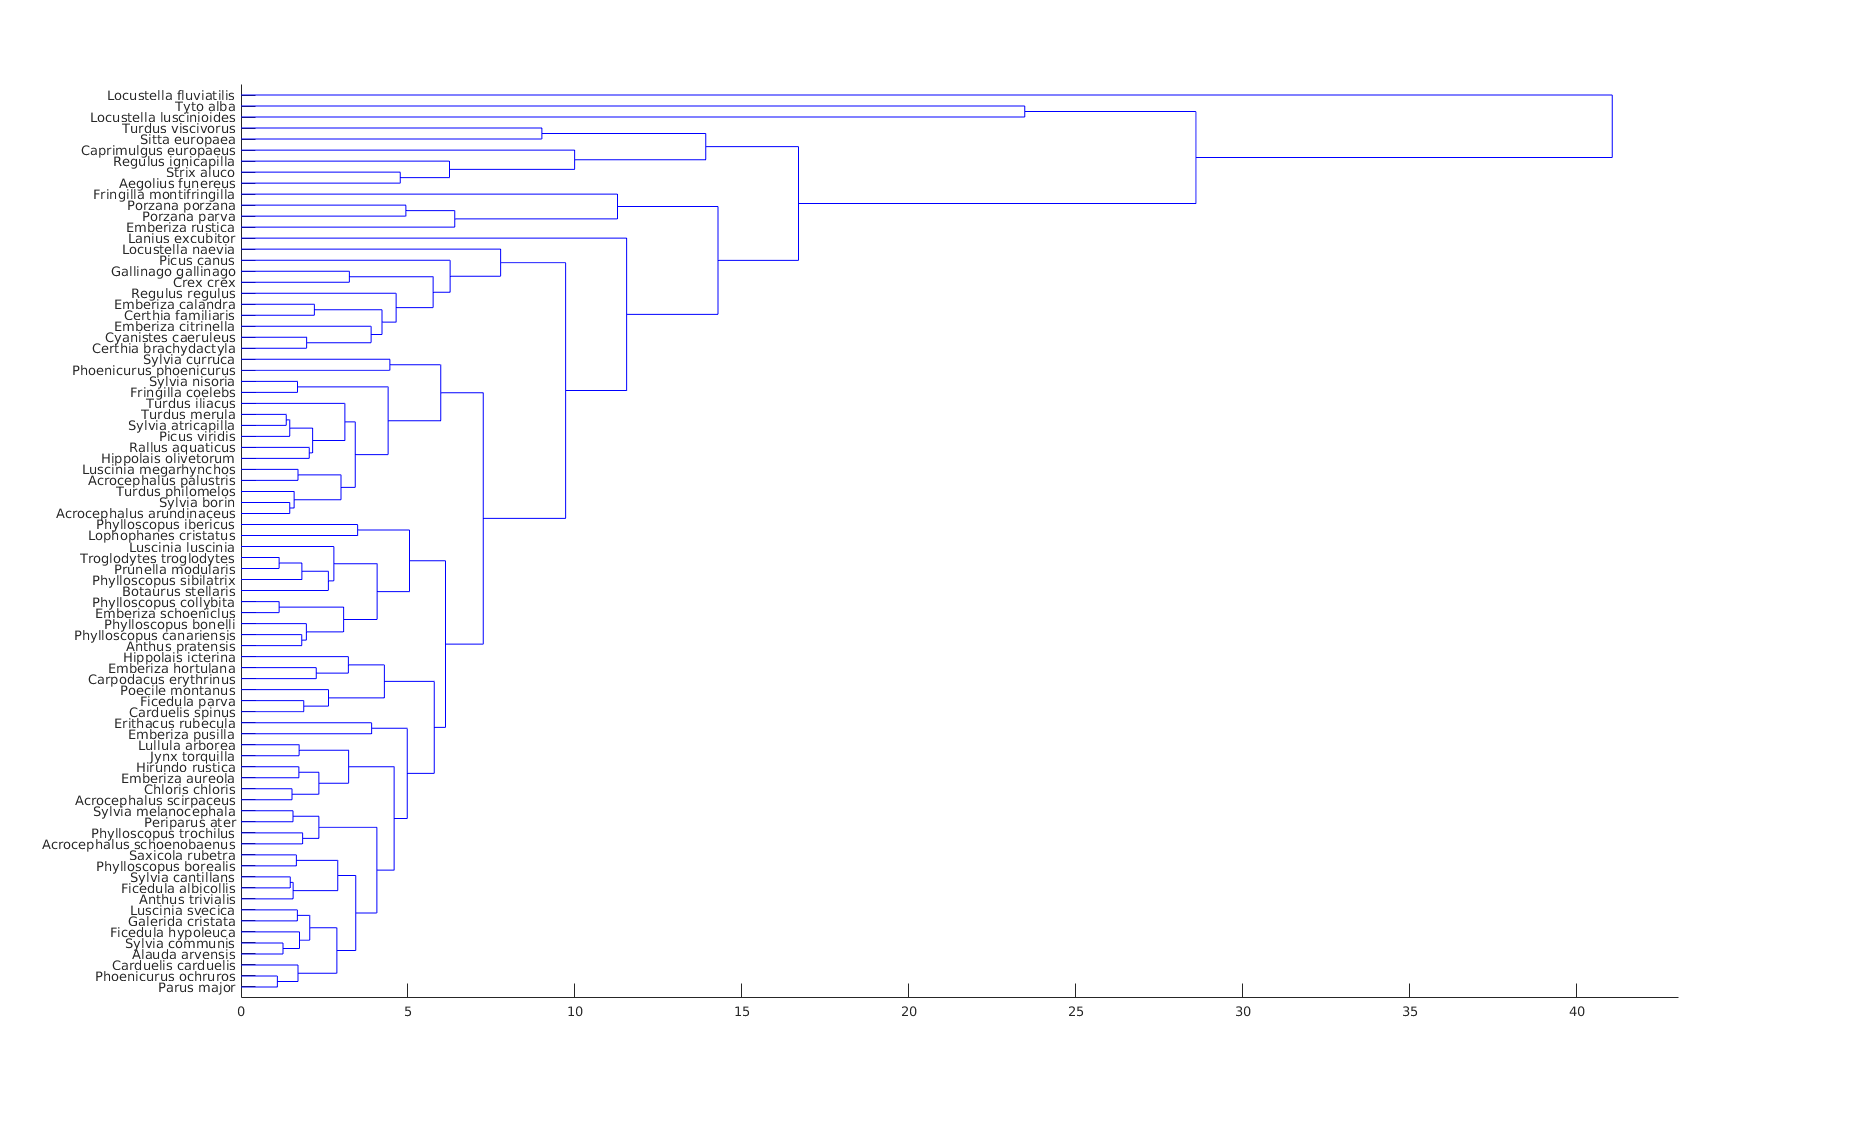
\includegraphics[width=\paperheight,height=18cm]{images/gmm_tree}}
    \caption{Phylo-acoustic tree generated using the Symmetric KL Divergence between pairs of emission models (GMMs) from HMMs.}
    \label{fig:gmmskld}
\end{sidewaysfigure}

\begin{sidewaysfigure}[!Ht]
\noindent\makebox[\textwidth]{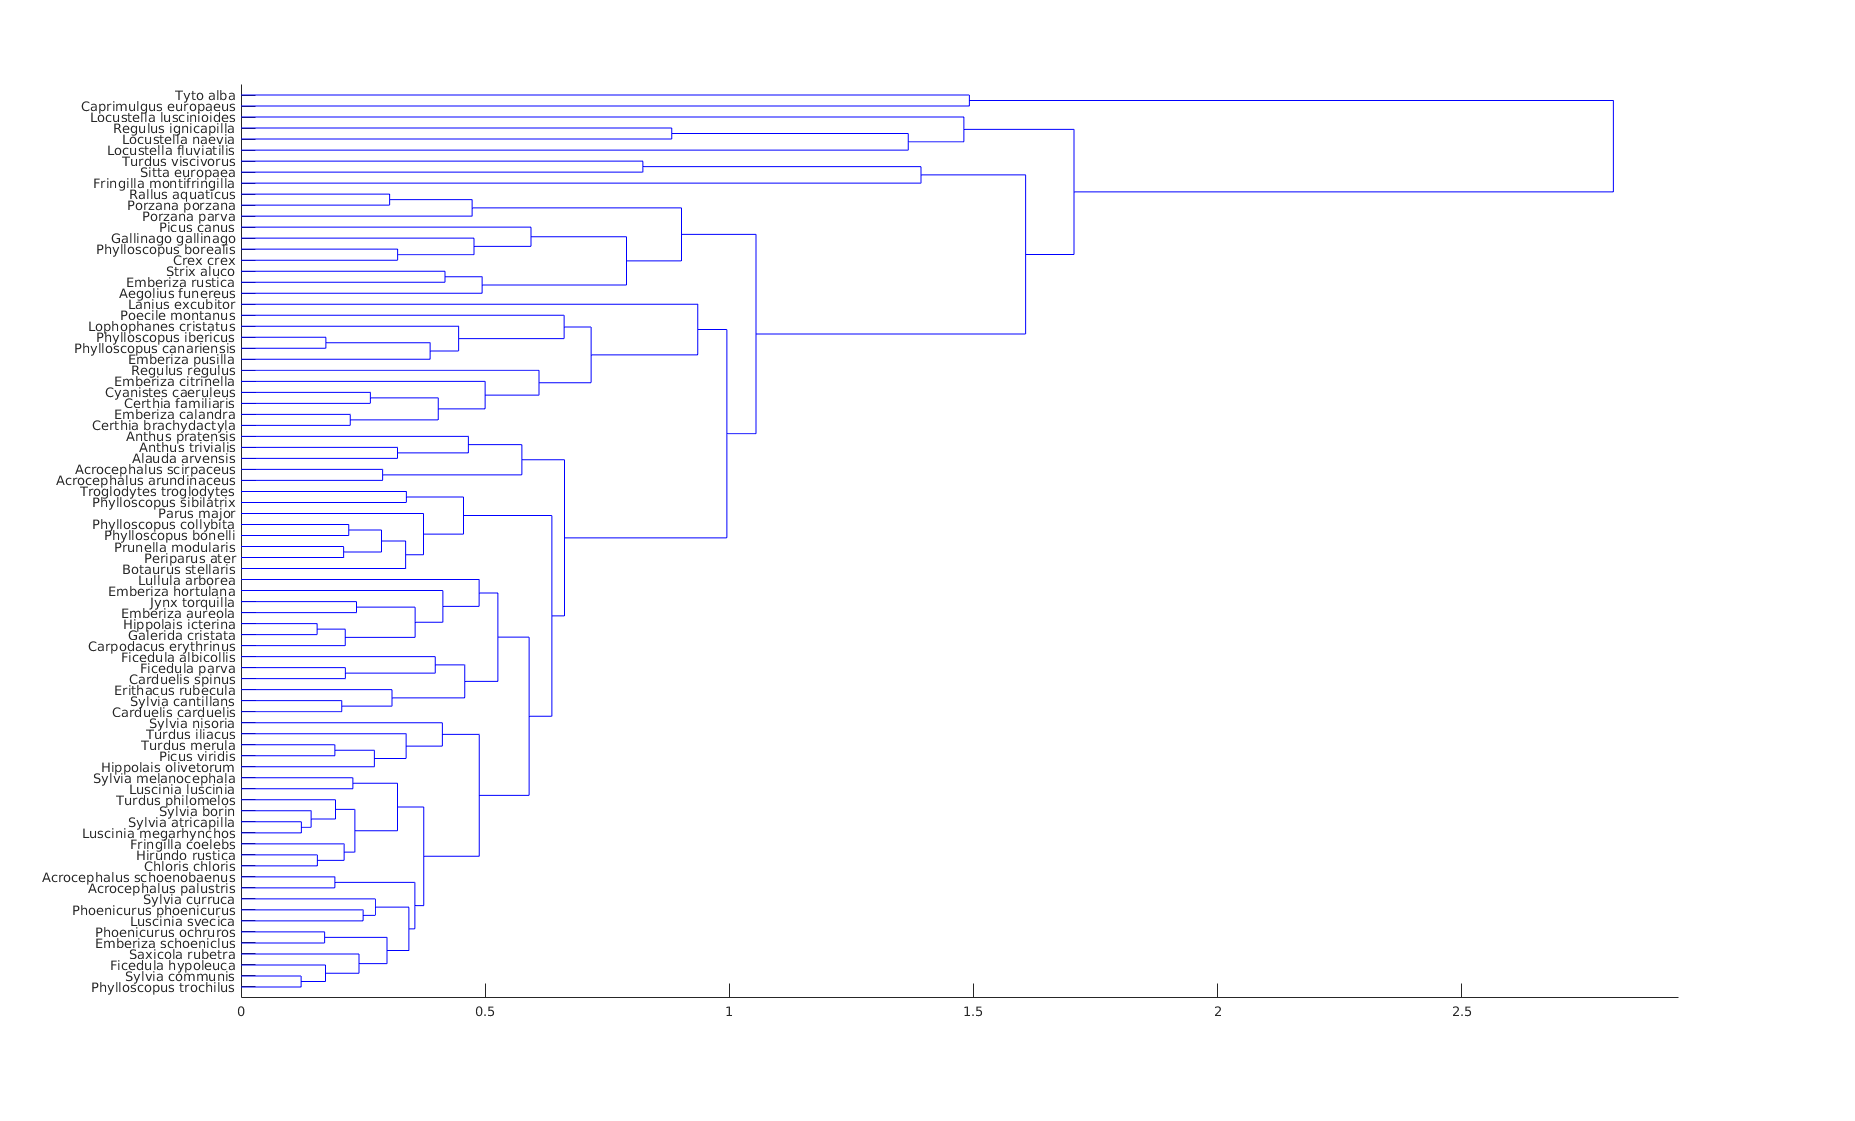
\includegraphics[width=\paperheight,height=18cm]{images/hmm_likelihoods}}
    %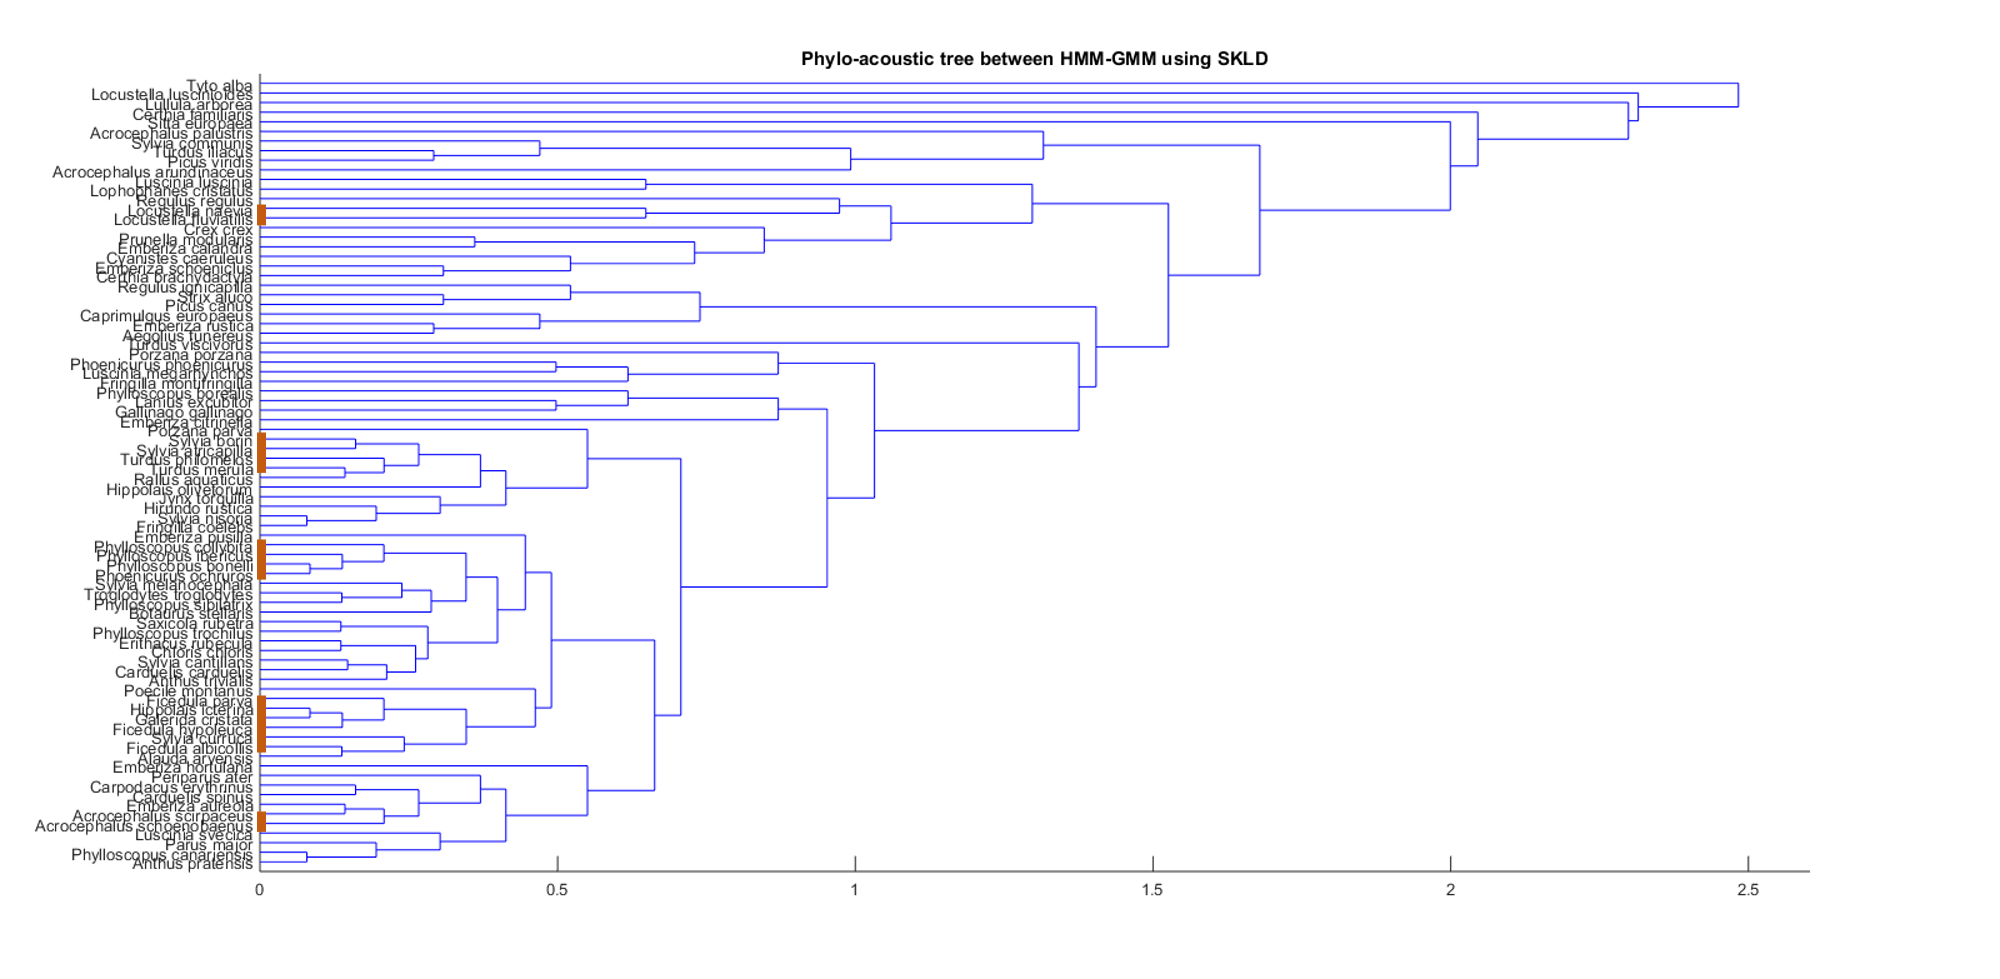
\includegraphics[width=\textwidth]{gmm_skld_2}
    \caption{Phylo-acoustic tree generated using the combined metric between HMMs.}
    \label{fig:hmmskld}
\end{sidewaysfigure}



\par Crucially, these trees are only meant to exhibit the acoustic relationships that exist across different bird species. Therefore, they are neither an equivalent to, nor are intended to replace other sorts of structures, particularly phylo-genetic trees. As discussed in Section \ref{section_introduction}, even if there is a link between birdsong and evolution, other exogenous factors such as migration patterns and geolocalisation may radically change bird vocalisations.
\par Instead, we are concerned by showing that the trees above do exhibit real structure (i.e. their shape is not coincidental). When there is real structure in data, clusters are tight and well separated from each other. This implies the distance between clusters becomes larger as smaller clusters merge. This maps visually to long branches in a dendrogram. On the other hand, when there is no real structure in data, objects tend to be about the same distance apart from each other (they are uniformly scattered in space). When a new cluster is formed in this scenario, linkage methods make a small contribution to the updated distance, since the original distances are already very similar. This translates into clusters that have a short lifetime.
\par In order to compare the structure of trees obtained from real and random data, we plotted the number of clusters $c(x)$ in each tree obtained after running Hierarchical Clustering up to lifetime $x$. This is a monotone decreasing function that is useful to contrast how quickly do clusters form as lifetime increases. As an example, see Figure \ref{fig_lifetime}.
\par We generated one such plot for each pair of trees $T_i, T_{i'}$. In both cases, we noted that the curves depicting the random statistical models drop to zero very quickly, since the resulting clusters live too little, as opposed to the real data models, whose clusters live many orders of magnitude longer. 

\clearpage

\begin{figure}[!t]
\centering
\begin{subfigure}{.5\textwidth}
  \centering
  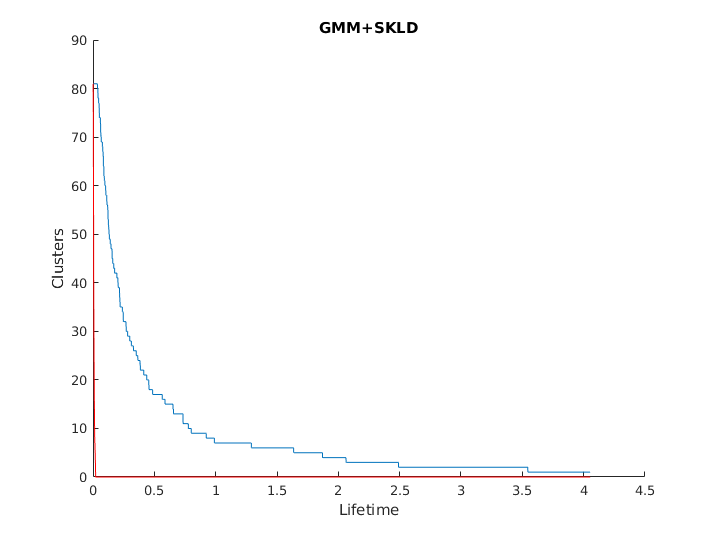
\includegraphics[width=\linewidth]{images/lifetime_gmm_skld}
  \label{fig:sub1}
\end{subfigure}%
\begin{subfigure}{.5\textwidth}
  \centering
  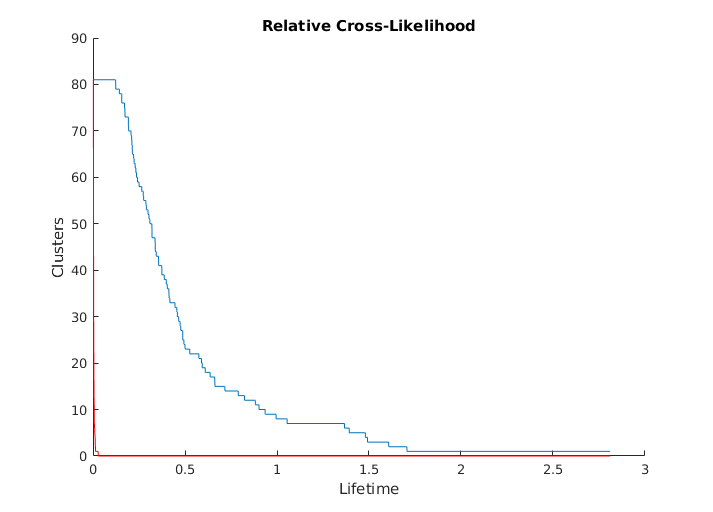
\includegraphics[width=\linewidth]{images/random_rcl}
  \label{fig:sub2}
\end{subfigure}
\caption{Lifetime vs. number of clusters after performing agglomerative clustering with GMM and SKLD (left), Relative Cross Likelihood (right). In both cases, the red (null hypothesis) curves approach zero very quickly compared with their real data counterparts. In both cases, the red curve approaches zero very quickly, suggesting that clusters are merged at a fast rate; on the other hand, the blue lines do not only span a longer lifetime, but they also contain short horizontal segments that grow longer as time flows. This suggests that it takes longer for clusters to merge as the number of remaining clusters decreases, which is consistent with our hypothesis: at the beginning, many clusters belong to the same community, and thus they are clustered fairly quickly. However, as communities are formed, they lie further apart from each other, and thus it takes longer for them to fuse. Likewise, the GMM+SKLD blue curve also has a steeper descent than the RCL one. This can also be seen when the divergence for each scenario is computed: a steeper descent translates into a smaller area under the curve, and thus a smaller divergence.
}
\label{fig_lifetime}
\end{figure}


%\begin{figure}[H]
%\centering
%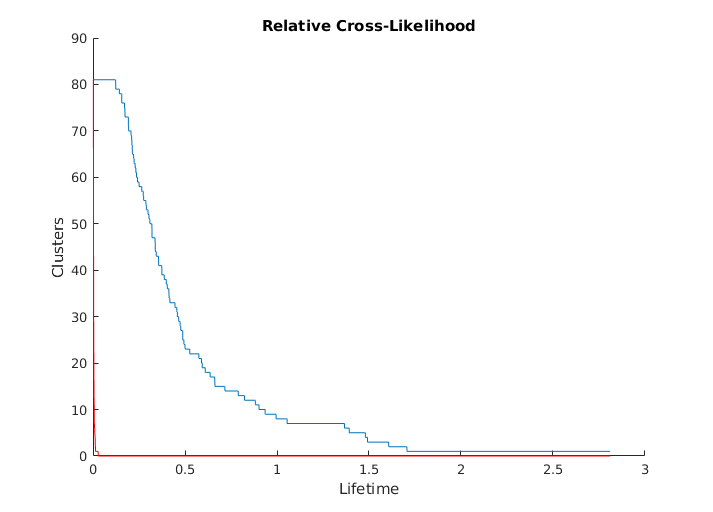
\includegraphics[width=11.5cm]{images/random_rcl}
%\caption{Lifetime vs. number of clusters after performing agglomerative clustering with Relative Cross Likelihood. Note the rate of change of the red curve (representing random structures) compared with the blue one (real data). The red curve approaches zero very quickly, suggesting that clusters are merged at a fast rate; on the other hand, the blue lines do not only span a longer lifetime, but they also contain short horizontal segments that grow longer as time flows. This suggests that it takes longer for clusters to merge as the number of remaining clusters decreases, which is consistent with our hypothesis: at the beginning, many clusters belong to the same community, and thus they are clustered fairly quickly. However, as communities are formed, they lie further apart from each other, and thus it takes longer for them to fuse.}
%\label{fig_lifetime}
%\end{figure}



\section{Conclusion}
\label{section_conclusion}
In this work, we introduced a length-invariant algorithm to build hierarchical structures from time series. This algorithm builds upon a functional view of our data, i.e. we trained statistical models for each of our classes, and then compared the models themselves via statistical metrics. Crucially, this higher-order view of our setting can be understood as a characterisation of the data's underlying manifold, which can then be further analysed using Hierarchical Agglomerative Clustering. Crucially, the length-invariance of our method makes it suitable to be applied in a wide range of domains. In particular, it can be extended to fields in which time series are required to be summarised disregarding their length.
\par We used our method to analyse acoustic relations across bird species in the British Isles by means of a hierarchical relational structure. Importantly, we were not aiming to challenge what evolution means from a biological perspective, but rather to show that there is a clear group structure in this set, and that we can show its existence by means of our method. Our results were evaluated by comparison with trees obtained from data sampled at random, i.e. we constructed so-called ``random trees" using the same algorithm, but feeding in uniformly distributed data. We observed that random trees have a very uniform structure in which objects tend to be about the same distance apart from each other, resulting in clusters with a very short lifespan - unlike real data trees, where species initially belong to well-defined clusters, which then have a long lifespan before finally being grouped together.
\par Remarkably, we also introduced a novel HMM similarity metric that accounts for all its emission and transition parameters in a concise fashion. This allows us to compare not only the observations contained in the time series, but also the time dynamics inherent to the model. Additionally, it is computationally efficient, since it only requires two more passes of the decoding phase (one for each cross-likelihood term) on top of those made during the training phase.
\par Future work includes applying this method to other domains, e.g. analysing the phonetic similarity of human languages by using our method over features extracted from human language excerpts, as well as using other visualisation techniques, such as multidimensional scaling, to further explore the manifold obtained through this method.

\section*{Acknowledgements}
The authors would like to thank the National Council for Science and Technology in Mexico (CONACYT) for funding this research project. 


\addcontentsline{toc}{chapter}{Bibliography}
\bibliographystyle{unsrt}
\bibliography{bib}

\end{document}


